

\subsection{Sharing \open and \closed between Searches}

We first describe how to share \open and \closed between the $k$ \astar searches of \kxastar under the assumption that all the heuristics $h_1, \ldots h_k$ are consistent, and relax this assumption later.

When the first \astar search in \kxastar (i.e., \astari{1}) starts, its \open contain $s$ and its \closed is empty, as in any standard \astar.
Then, when \astari{1} finishes its search (with an optimal path to $t_1$), it passes \open and \closed to \astari{2}.
This includes the $g$ value of all the nodes generated by \astari{1}, and in some implementations also their $h$ values.\footnote{While it is possible not to store the $h$ value of a state and re-compute it every time the search needs the $f$ value of that state, standard implementation [[AF: standard? maybe time aware? BTW, you store the f value because open is sorted accordingly. And if you also know g then you know h too because f=g+h.]] of \astar usually stores the $h$ value of every generated state to save heuristic computation time.} 
If \closed contains $t_2$, we can halt since all the heuristics are consistent.[[AF: and $g(t_2)$ cannot decrease]]
Otherwise, we re-compute the $h$ and $f$ values stored for the states in \open using $h_2$ and $g+h_2$, respectively, and reorder these states to [[AF: in]] \open according to their up-to-date $f$ values.
This step is needed since the states were previously ordered in \open according to $f$ values computed with $h_1$.
Note that even if $t_2$ is in \open, we must still continue the search to verify that the optimal path to it has been found.
Then, the search continues as a regular \astar until $t_2$ is expanded.
This process continues, passing \open and \closed from \astari{2} to \astari{3} and so on, until all $k$ states have been expanded.

Now, consider the case where the heuristics $h_1, \ldots h_k$ are admissible but not consistent.
In this case, when passing information from \astari{1} to \astari{2} it might be the case that $t_2$ has been expanded and is currently in \closed, but the optimal path to it has not been found yet.
[[ADD EXAMPLE FROM THE POWER POINT]][[AF: this is easy to understand. No need for an example in my opinion]]
Thus, if the heuristics are inconsistent then having $t_2$ in \closed supplied by \astari{1} is not a sufficient condition to ensure admissibility of the search (i.e., finding an optimal path to $t_2$).
In order to guarantee optimality, the $h$ and $f$ values of all the states in \open must be re-computed using $h_2$ and \open must be reordered according to these up-to-date $f$ values.
Then, the search can halt only when it is guaranteed that the $g$ value of $t_2$ is indeed optimal. This will be true either when $t_2$ is expanded or when the minimal $f$ value in \open is larger than or equal to the $g$ value of $t_2$.

[[Roni: maybe worthwhile to say all this more formally, maybe not. No, this is OK]]
[[Roni: maybe noting that we can't do lazy here? Lazy was not yet defnied]]

%Advantages 
Sharing \open and \closed in \kxastar can be beneficial because a state is only generated once, even if it is manipulated by more than one of the \astar searches, and the $g$ values of states get more accurate as we perform more searches and gain better knowledge of the search space.
More accurate $g$ values leads to more accurate $f$ values and to potentially expanding fewer states. [[Roni: is an example needed? AF: no need for an example. Relatively easy.]]

%Disadvantages 
However, sharing \open and \closed in \kxastar can also hurt performance.
%[[Roni: can this happen also with consistent heuristics, I believe so]]
\begin{itemize}
\item Memory consumption may increase since \open and \closed include all states generated or expanded by all the $k$ \astar searches.
%- For any $1<i\leq k$, \closed of search \astari{i} may contain states that are surplus for $\Pi_i$,  and \open may contain states that that \open for \astar run
\item Runtime may decrease [[AF: increase??]], since \open operations (insert, pop, reorder) now may work on a larger set of states
\item Runtime may decrease  [[AF: increase??]], since for $1<i\leq k$ we compute $h_i$ for every state in \open, including states from past searches.
Such states may not even be generated by \astari{i}, and thus computing $h_i$ for them is redundant.
[[Roni: I need some term like surplus states but for generated states. There is something like this I think in Meir's work?]]
\end{itemize}

\abda{Add an example for poor max-memory usage.}[[AF: I do not think that an example is needed. Everything here is easy]]

The last item is especially problematic, since heuristic computation can be very time consuming.
Thus, we propose the following \kxastar variant that shares some information between the searches but not all of it.

[[AF: you might want to give a name to this straightforward variant. Like "KxA-trivial-sharing"]















%[[AF: are you moving now to kA* or is this yet another versin of kxA*, please give a nice connecting sentence or sentences]]

%Sharing information between searches highlights the importance of how we order the goals. In the absence of an intelligent heuristic to choose this order, an alternative can be to search for all the goals in parallel. This can be done either with multiple CPUs or even on a single CPU in a round-robin manner, expanding in each iteration a node from a different \astar search, i.e., from a different \open.

%Again we are faced with the question of which information to share between the searches. One option is to only share $g$ values, as suggested above for the sequential search. This means there are $k$ \astar searches, each maintaining a separate \open and \closed, but when a state's $g$ value gets updated, the updated $g$ value is used by all the $k$ searches.

%[[AF: the above was how to perform parallel g-sharing A*. Right, next you talk about how to perform parallel f-sharing A* and this gives birth to kA*.]]

%The second information sharing option described in the previous section is to share \open and \closed. This can be done as follows. When a state is popped out [[AF: expanded, or chosen for expansion]] by one of the $k$ searches, it is removed from all the \open{}s of the $k$ searches, and the states generated by expanding this state are added to all the \open{}s, each  with its corresponding heuristic function.

%We describe two ways to do so in this context of searching in parallel for all goals. The first is to have $k$ separate \open{}s, one per goal, and each ordered according to the corresponding heuristic function. When a state is popped out by one of the $k$ searches, it is removed from all the \open{}s and all the generated children are added to all \open{} with the corresponding heuristic function for each \open. 


%: \begin{itemize}
%\item {\bf $k$ synchronized \open{}s.} In this option,  there is a separate \open for each of the $k$ goals, and each \open is ordered according to the corresponding heuristic function. When a state is popped out by one of the $k$ searches, it is removed from all the \open{}s and all the generated children are added to all \open with the corresponding heuristic function for each \open{}.
%\item {\bf $k$ synchronized \open{}s.} In this option,  there are $k$ \open{}s, one per goal. When a state is popped by one of the $k$ searches, it is removed from all \open{}s and its children  \item {\bf One joint \open.} In this option there, is single \open for all $k$ searches.  \end{itemize} having $k$ separate but synchronized \open{}s, and having a single joint \open.  The first option

%Another option is to also share \closed and maintain $k$ \open{}s. When a node is generated, it needs to be inserted to all $k$ \open{}s, where each \open is sorted according to the $f$ value for its corresponding goal. 
%Here too, the advantage of the first option is that we get better $g$ values and thus a better ordering of (all of the $k$) \open{}s. The disadvantage is that the same node can be generated multiple times for different searches. 
%The advantage of the second option is that nodes are generated only once, but we maintain $k$ copies of every generated nodes in each of the $k$ \open{}s. However, in every \open we only store pointers and $f$ values, 
%while the $g$ value and the data structure holding the state that the node represents is only stored once. 

%[[TODO: EXAMPLE TO CLARIFY, DEEPER DISCUSSION ON DIFFERENT OPTIONS]]

%When searching for the goals in parallel, there is actually a third option: sharing \closed and have a single joint \open. [[AF: it is not a third (new) option, there is no point in storing different open lists. So, you merge them into one open list and KA* is now born.]] We call this third option \kastar, and describe it next.


%[[AF: so, you have 5 algorithms, basic kxA* (no sharing), g-sharing KxA*, f-sharing KxA* and parallel g-sharing KxA*. The parallel f-sharing KxA* is in fact kA* which deserves a new section. I hope you like this and use names for these algorithms. At least give then variant numbers V1, V2 etc.]]


Before presenting a complete pseudo code for \kastar, we highlight several aspects that differentiate it from \kxastar.

%needs to ... per node As a consequence of sharing \open and \closed, \kastar needs to ... per node. This value is based on the distance to start as well as all available heuristic information. 

\subsection{$k$ Heuristics per Node}

In \kxastar, there are $k$ searches, where in every search considers a single heuristic function. In \kastar, there is a single search, but that search considers $k$ heuristic functions, one per goal. 
Mathematically, \kastar computes for every generated node $n$ a $k$-ary vector $\vect{h}(n) = \tuple{h_1(n), \ldots h_k(n)}$, where $h_i(n)$ is the heuristic estimate of the cost to get from $n$ to goal $t_i$. Then, \kastar uses a \emph{heuristic aggregation function}, $\Phi$, to combine these $k$ heuristic values with the $g$ value into a single value $F(n) = g(n) + \Phi(\vect{h}(n))$. 



%\kastar uses $F$ to choose which node to expand in every iteration. 

%\astar considers a single heuristic value $h(n)$, while \kastar can consider $k$ heuristic values, one per goal. Mathematically, \kastar computes a $k$-ary vector $\vect{h}(n) = \tuple{h_1(n), \ldots h_k(n)}$, where $h_i(n)$ is the heuristic estimate of the cost to get from $n$ to goal $g_i$. Then, \kastar uses a \emph{heuristic aggregation function}, $\Phi$, to combine these $k$ heuristic values with the $g$ value into a single value $F(n) = g(n) + \Phi(\vect{h}(n))$. \kastar uses $F(n)$ to choose which node to expand in every iteration. 

%. \kastar is a best-first search using this single $F$ value, i.e., in every iteration, the node with the minimal $F$ value is expanded. 
%then used to determine which node to expand next, 

We discuss in Section~\ref{sec:aggregating} the underpinnings of the heuristic aggregation, but in the meantime one can take $\Phi(\tuple{h_1(n), \dots h_k(n)}) = \min_{i\in[1,k]} h_i(n)$ or $\Phi(\tuple{h_1(n), \dots h_k(n)}) = \max_{i\in[1,k]} h_i(n)$ as reasonable instantiations. 
The $F$ value is used to prioritize nodes ready to be expanded.
That is, in every iteration \kastar selects from \open a node with the smallest $F$ value. 








%Thus, the computational effort of generating a node in \kastar is larger than in regular \astar, as it requires computing $k$ heuristic values. 

%\footnote{As discussed later in the paper, the actual computational cost in \kastar can be smaller, since as the search progresses the list of relevant goals becomes smaller, and consequently computing $F$ becomes easier.}

\subsection{Maintaining the Set of Active Goals}

When a goal is expanded in \astar, the search halts.
By contrast, in \kastar the search does not halt until a lowest-cost path to each of the $k$ goals has been found.
To this end, \kastar tracks the set of goals that have not been expanded yet. 
%for which a lowest-cost path has not been found.
This set of goals is referred to as the set of \emph{active goals}.  
%[[AF: use this term above when saying that a search notifies later search that their goal was found]].
Maintaining the set of active goals is also used to avoid redundant heuristic computations: when a node is generated we compute the heuristics only for goals that are still active. %This idea  may create further enhancements which are discussed in Section~\ref{sec:lazy}.
To this, end we extend the previous notation by having $\Phi$ accepts vectors of different sizes, and provide it only the heuristics for the active goals when generating a node. 

%defining $\Phi[AG]$ as an aggregation function that only aggregates over the values that correspond to the set of goalsset $AG$ can accept vectors of different sizes, specifically any size between 1 and $k$, and only  Common aggregation functions such as $\max$, $\min$, and average are all such functions, as we can apply them to vectors of different sizes. 
%5[[TODO: New subsection to read]] Next, we ask the question of which heuristic aggregation functions can use Lazy \kastar and obtain  an admissible results (i.e., optimal paths to all goals). [[AF: I would summarize that eager and eager+ are always good. Lazy is OK for min but not for max. And now, we want to know what further with other functions]] To this end, we somewhat abuse [[AF: is this the correct word? You now use it on any size of vector up to k. Maybe you are widening it? Generalizing?]] the previous notation by defining $\Phi$ as an aggregation function that can accept vectors of different sizes,  specifically any size between 1 and $k$. % Common aggregation functions such as $\max$, $\min$, and average are all such functions, as we can apply them to vectors of different sizes. 




%\subsubsection*{Node evaluation function.} When searching for a single lowest-cost path with \astar, the state are popped from \open according to their $f=g+h$ values. In \kastar, we compute the $h$-value forand associate every state in \open with a value that considers the $h$-value for each of the $k$ goals.     Thus, when a state is generated then we compute the heuristic for each of the $k$ goals.

$\vect{h}(n)\gets \tuple{ h_i(n) \mid i\in ActiveGoals }$
$F\gets g(n)+\Phi(\vect{h}(n))$







%[[AF: In line 23, don't you want to return some of the paths if you have them?]]\roni{I think this will just confuse. The problem is defined for all the $k$ paths.}
\subsection{Summary}
[[TODO: New subsection to read]]
\begin{figure}
\centering
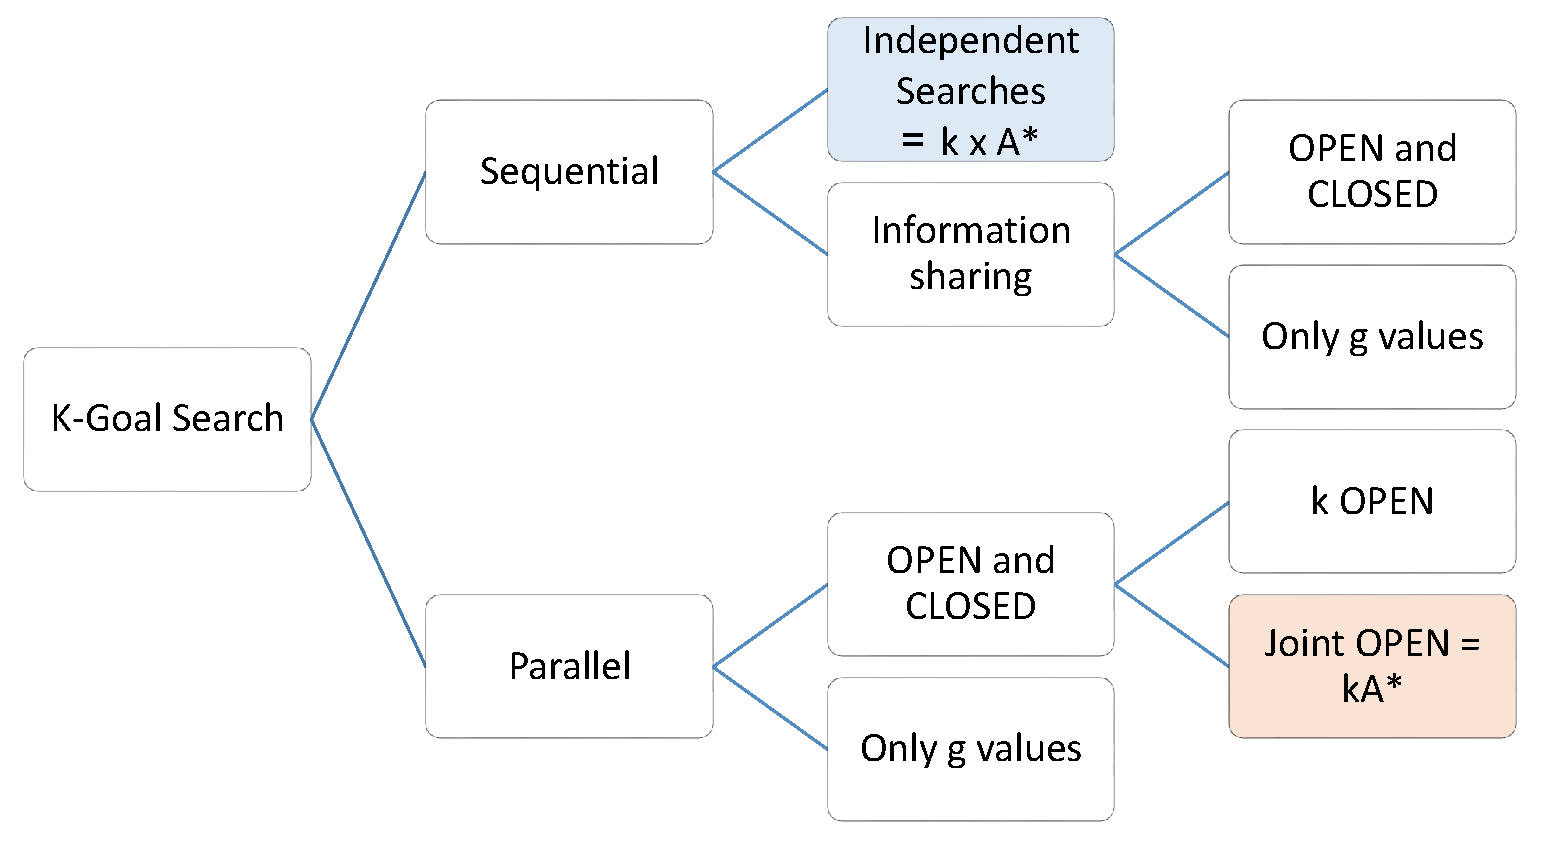
\includegraphics[width=0.8\textwidth]{k-goal-approaches}
\caption{A visual illustration of the different approaches we describe for solving \kgs.}
\label{fig:approaches}
\end{figure}

To summarize the discussion so far, we proposed two general approaches for solving \kgs: searching for optimal paths to the $k$ goals sequentially, one goal at a time, and searching for all $k$ optimal paths in parallel.
In each of these approaches, there is a question of how much information is shared between the searches: one can choose not to share any information between the searches, to share only the most up-to-date $g$ values, and to share also \open and \closed.
Specifically in the parallel search approach, there is no point in not sharing any information between the searches, and there are two options to share \open and \closed: either by maintaining $k$ \open{}s and synchronizing them, or by maintaining a single \open that aggregates in some way the information from all heuristics.
Figure~\ref{fig:approaches} illustrates all these approaches and variants for solving \kgs.
Other variants of this may also exist.

What we have not described yet is how does the parallel search with a single \open aggregates the heuristic values for all goals, and how does the sequential searches choose which goal to solve first. In this work we focus on answering the first question.

[[AF: This is indeed a summary and maybe it can be merged above somehow because there is repetition of text. Anyhow, it would be great to give a name to each of them or at least a sequential number.  And, there is a separation between everybody who only share information to KA* which uses one OPEN. This must be clear]]